\documentclass[aspectratio=169,dvipsnames]{beamer}
\beamertemplatenavigationsymbolsempty
% \documentclass{beamer}

% UNCOMMENT FOR HANDOUTS
% \usepackage{pgfpages}
% \pgfpagesuselayout{2 on 1}[landscape,letterpaper,border shrink=5mm]
% \setbeameroption{show notes}

\mode<presentation>
\usetheme{Boadilla}
\usecolortheme{spruce}
\usepackage{../../LizStyle,ulem}
\usepackage{color}
\usepackage[color,matrix,arrow]{xy}
% \input xy
% \xyoption{all}
\usepackage{tikz}
\usepackage{tikz-cd}
\tikzset{commutative diagrams/diagrams={ampersand replacement=\&}}

\AtBeginSection{\frame{\sectionpage}}


% ==========Command for putting comments and removing them=======
% Visible:
\newcommand{\InstructorNotes}[1]{{\color{orange}#1}}
\newcommand{\InstructorList}[1]{
\begin{itemize}
	\color{orange}
	#1
\end{itemize}
}
% Removed: JUST COMMENT OR UNCOMMENT THIS
 %\renewcommand{\InstructorNotes}[1]{}
%\renewcommand{\InstructorList}[1]{}
% %

\newcommand{\bvfill}{\vskip0pt plus 1filll}

\usepackage{multimedia}
\usepackage{graphbox}

% \usepackage{algpseudocode}


\newcommand{\Reeb}{\textbf{Reeb}}
\newcommand{\Rtopc}{\textbf{Rtopc}}
% \newcommand{\RR}{\mathcal{R}}

\newcommand{\Set}{\textbf{Set}}
\newcommand{\Vect}{\textbf{Vect}}
\newcommand{\Top}{\textbf{Top}}
\newcommand{\Int}{\textbf{Int}}


\graphicspath{ {Figures/} {../Figures/}{../../Figures/} }



\begin{document}
%\pdfoptionpdfminorversion 5
%\logo{\includegraphics[height=1.5cm]{dukeshield.pdf}}
\title[Lec 2]{Ch 2.1: What is Statistical Learning?}
\subtitle{Lecture 2 - CMSE 381}
\date{Weds, Jan 14 , 2026}



\institute[MSU-CMSE]{Michigan State University\\
			::\\
          Dept of Computational Mathematics, Science \& Engineering}
%\author[Dr.~Bao]{Prof.~Lianzhang Bao}

\begin{frame}
 \titlepage


\end{frame}
%--------------------------
\begin{frame}[t]{Announcements}
	\begin{columns}
	\column{.4\textwidth}
	\centering
	
	\textbf{Last time:}
	\begin{itemize}
		\item Discussed where to find everything
		\begin{itemize}
			\item Course webpage 
			%\item Slack 
			\item D2L
		\end{itemize}
		\item Check out the syllabus!
	\end{itemize}

	\vspace{.2in}

	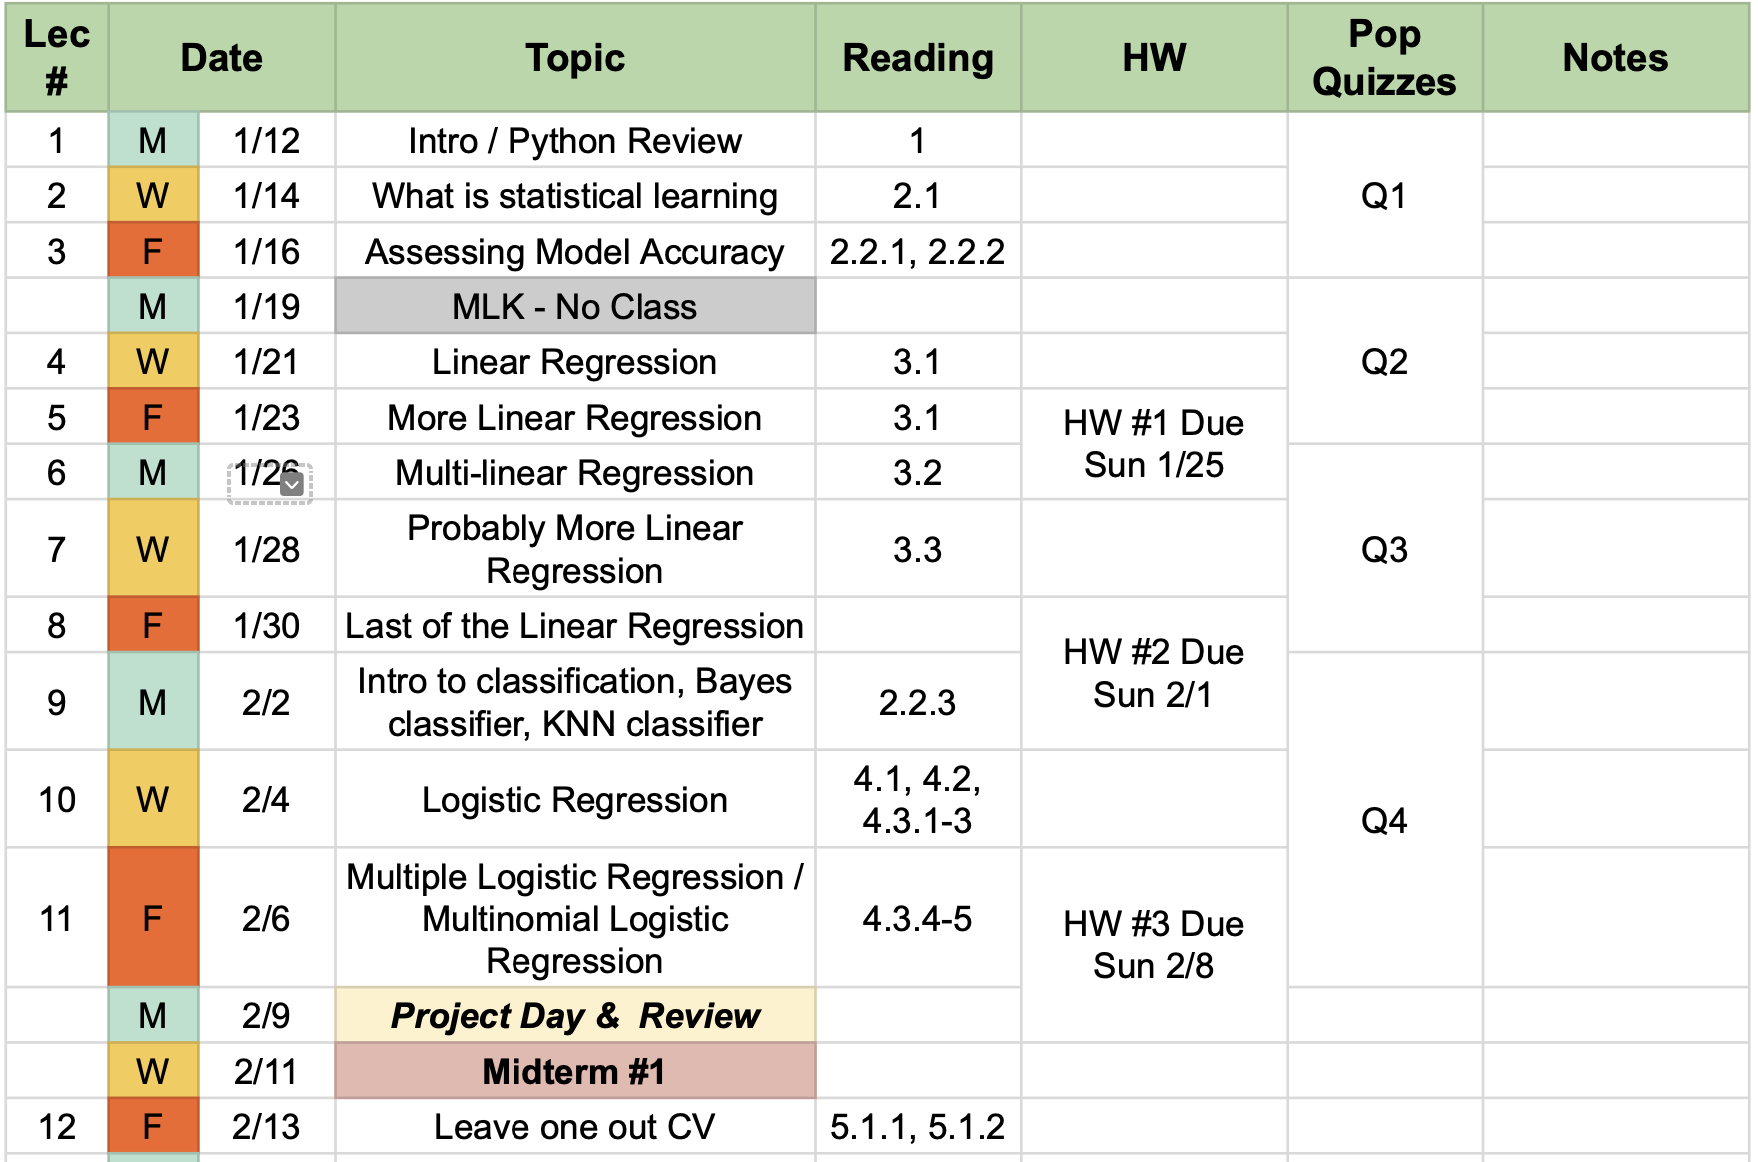
\includegraphics[alt={screenshot of course class schedule for lectures 1 to 12},
	align = c, width = \textwidth, trim = 0 200 0 0, clip]{Schedule-S26-1.png}
	
	\column{.4\textwidth}

	\textbf{Announcements:}
	\begin{itemize}
		%\item Get on slack!
		%\begin{itemize}
			%\item +1 point on the first homework if you post a gif in the thread
		%\end{itemize}
		\item First homework due Sun Jan 25
		\item First office hours next week
	\end{itemize}
	\centering
	\end{columns}
\end{frame}
%--- Next Frame ---%
\begin{frame}[c]{Covered in this class}

\begin{columns}
\column{.4\textwidth}
\centering
\begin{itemize}
	\item Input/output variables
	\item Prediction vs inference
	\item Reduceable vs irreduceable error
	\item Overfitting
	\item Classification vs regression
	\item Supervised vs Unsupervised learning

\end{itemize}

\column{.4\textwidth}
\centering
\begin{itemize}
	\item Please note: no jupyter notebook for today's class, slides only
\end{itemize}

\end{columns}

\end{frame}
%--- Next Frame ---%

\begin{frame}[t]{An example data set: \texttt{Advertising}}
\begin{columns}
\column{.28\textwidth}
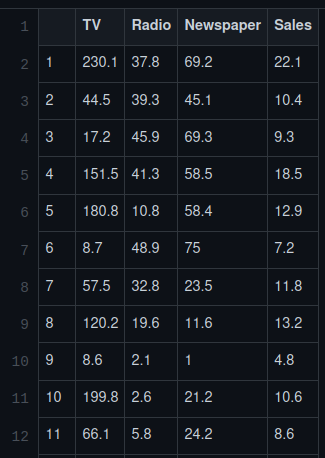
\includegraphics[alt={screenshot of the advertising data set},width=\textwidth]{AdvertisingDataSet-Screenshot.png}
\column{.6\textwidth}
\begin{itemize}
	\item Sales of a product in 200 markets, along with amount spent on three differnt types of advertising
	\item Goal: \InstructorNotes{Predict Sales based on amount spent in each type of advertising}

	\item Input variables: \InstructorNotes{TV, Radio, Newspaper}
	\item Output variable: \InstructorNotes{Sales}
\end{itemize}

\vspace{1in}

\end{columns}

Data available at \href{https://msu-cmse-courses.github.io/CMSE381-S26/DataSets/DataSets.html}{msu-cmse-courses.github.io/CMSE381-S26/DataSets/DataSets.html}
% \url{https://github.com/nguyen-toan/ISLR/blob/master/dataset/Advertising.csv}
\end{frame}
%--- Next Frame ---%

\begin{frame}[c]{Notation and Big Assumption}

\begin{columns}
\column{.4\textwidth}
Input variables: $X_1,X_2,\cdots,X_p$

Output variable: $Y$
\column{.4\textwidth}
{\Large
\begin{equation*}
	Y = f(X) + \e
\end{equation*}
}

\InstructorList{
	\item $f$ is the systemic information that $X$ provides about $Y$. 
	\item It is the ground truth that we want but can't access 
	\item So our goal is to come up with an estimated model $\hat f$.
	\item $\e$ is a random error term which is independent of $X$ and has mean 0
}

\end{columns}



\end{frame}
%--- Next Frame ---%


\begin{frame}[t]{\texttt{Advertising} Example}
	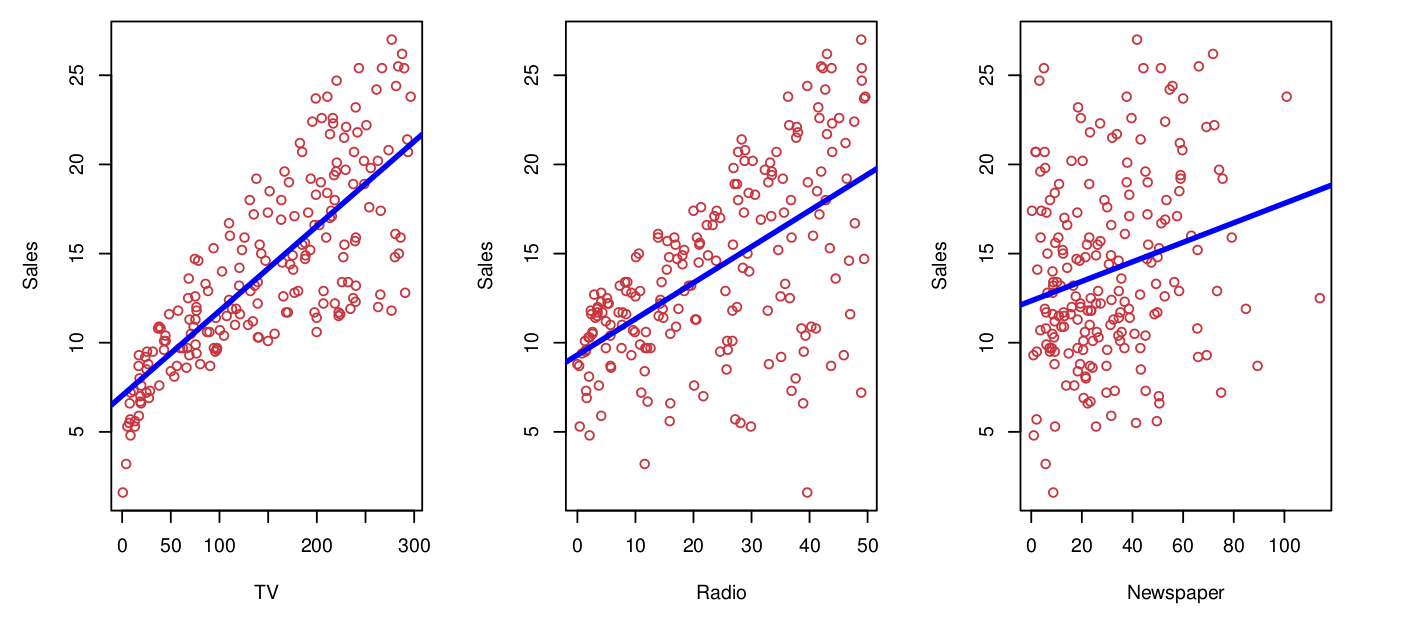
\includegraphics[alt={Sales versus TV, radio, and newspaper advertising spending all in units of 1000},width=\textwidth]{Fig2-1}
\end{frame}
%--- Next Frame ---%
\begin{frame}[c]{More examples}

\begin{columns}
\column{.55\textwidth}
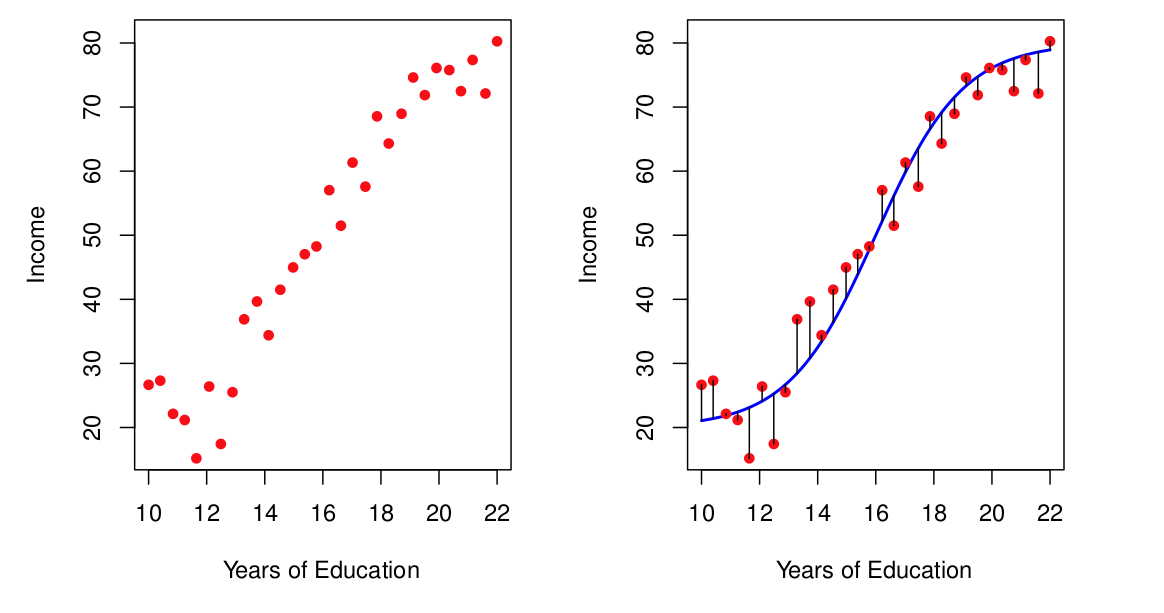
\includegraphics[alt={Data points for income in units of 1000 versus years of education and a nonlinear curve fit to the data},width=\textwidth]{Fig2-2}
\column{.4\textwidth}
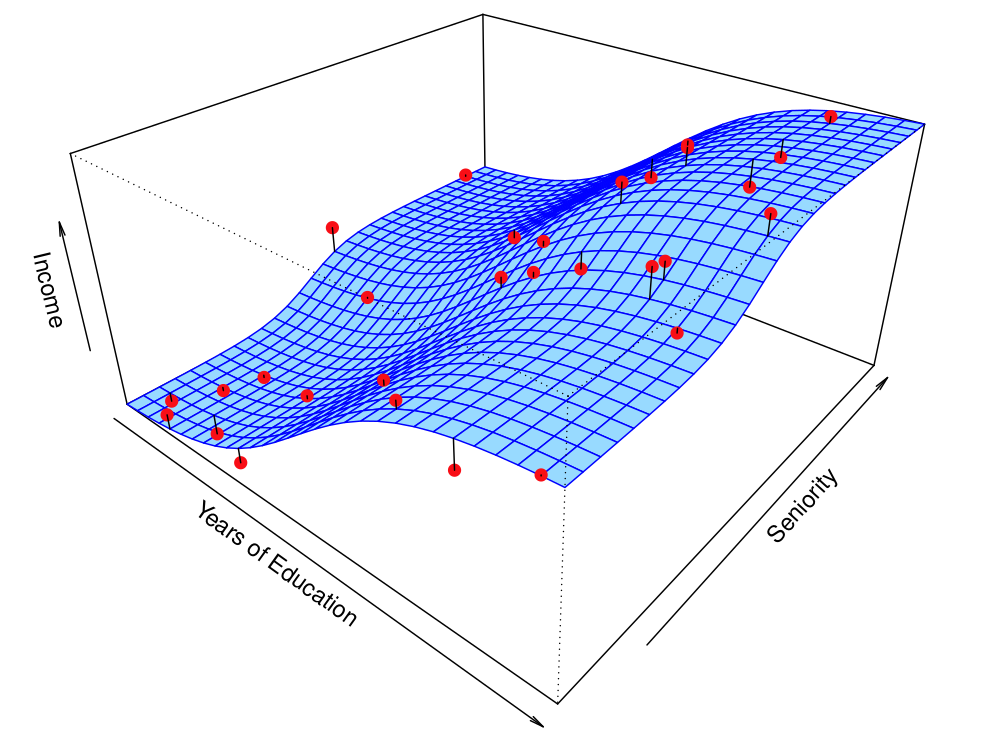
\includegraphics[alt={Data points for income in units of 1000 versus years of education and seniority along with a surface fit to data},width=\textwidth]{Fig2-3}

\end{columns}

\end{frame}
%--- Next Frame ---%
\section{Prediction vs Inference}


\begin{frame}[c]{Prediction}

\begin{columns}
\column{.4\textwidth}

Given a value $X$, try to provide an estimate for $f(X)$. 

Build a model:
{\Large
\begin{equation*}
	\hat Y = \hat f (X)
\end{equation*}}
\InstructorList{
  \item Want to get a good guess for $f$, which is unknown blue 
  \item Model is $\hat f$ is green dashed lines
%   \item Error is how far off prediction $\hat Y$ is from what actually happened
}

\column{.4\textwidth}
Example: If we spend \$250 on TV advertising, what do we predict we will we make in sales?

	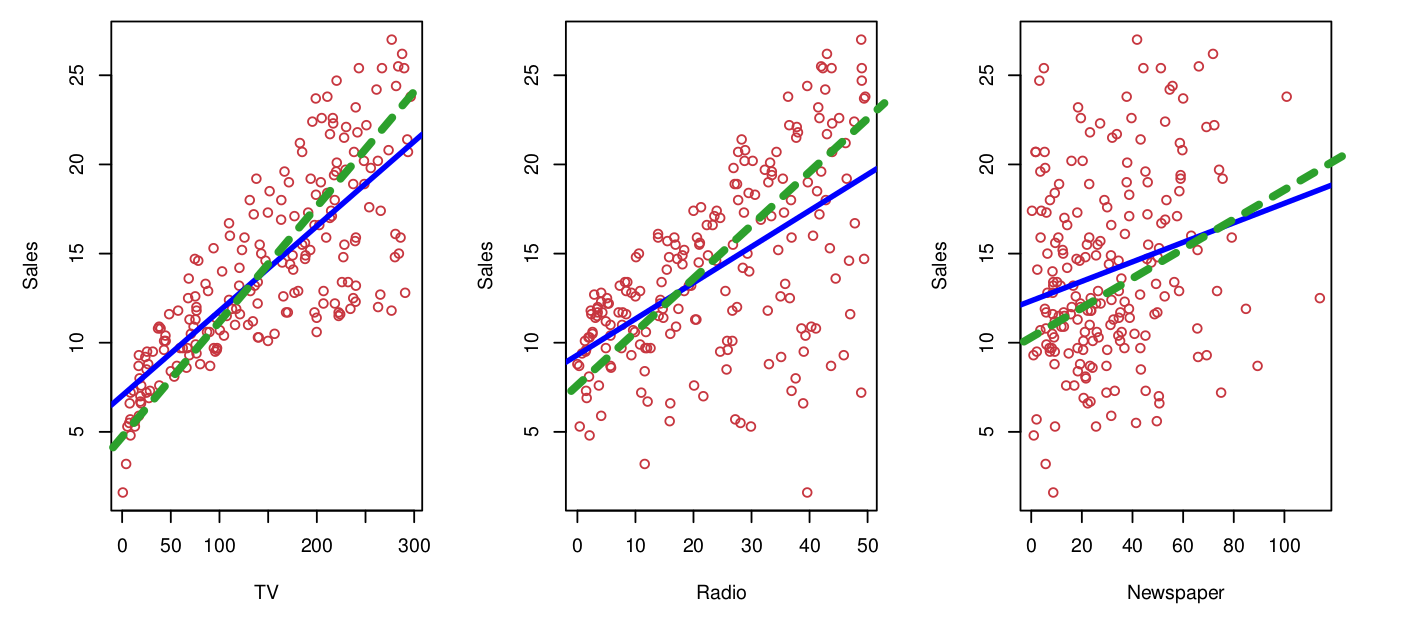
\includegraphics[alt={Sales versus TV advertising spending in units of 1000 along with two different linear fits},width=.7\textwidth,trim = 0 0 700 0, clip]{Fig2-1-WithHatF}
\end{columns}

\end{frame}
%--- Next Frame ---%
{
  \setbeamercolor{background canvas}{bg=Apricot!25}
\begin{frame}[t]{Group question:}
\begin{columns}
\column{.25\textwidth}
\centering


% \includegraphics[align = c, width = \textwidth]{}

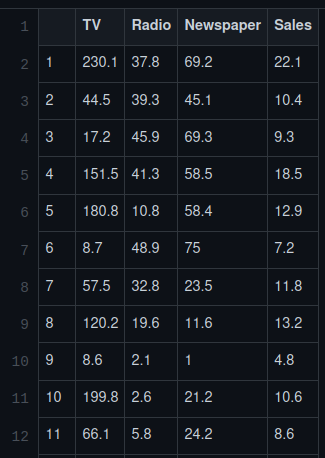
\includegraphics[alt={screenshot of the advertising data set},
width=\textwidth, trim = 0 300 0 0, clip]{AdvertisingDataSet-Screenshot.png}

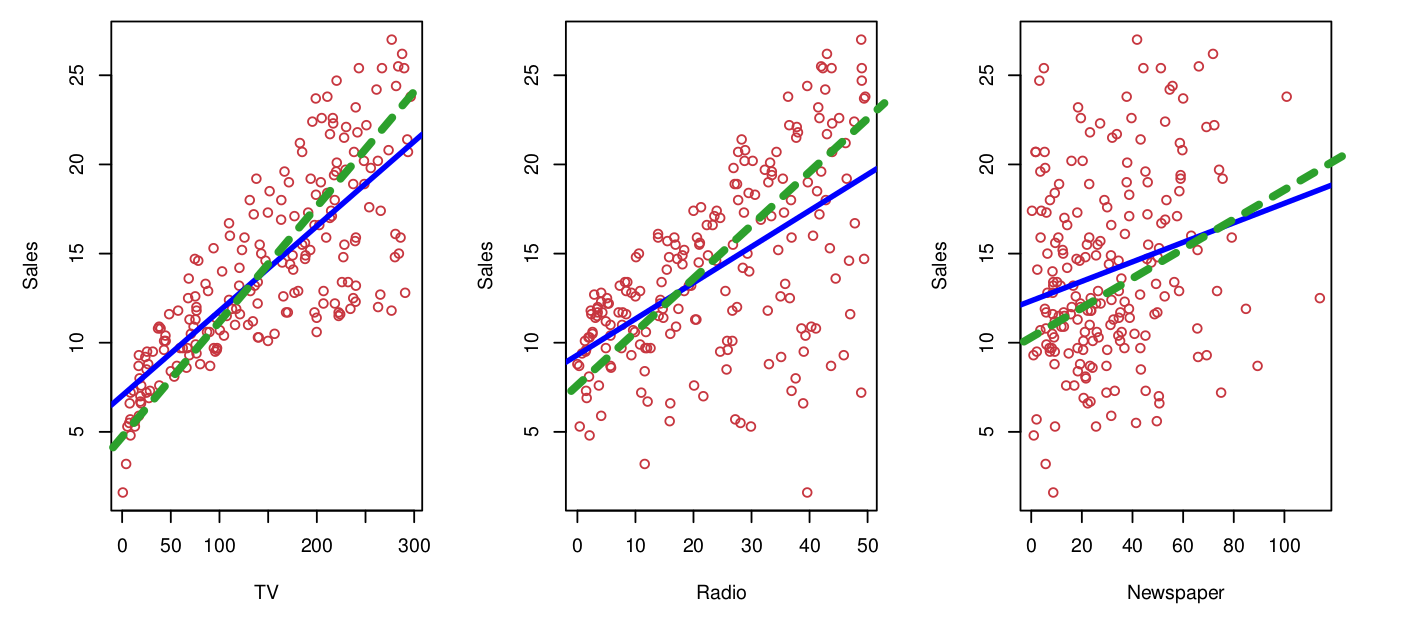
\includegraphics[alt={Sales versus TV advertising spending in units of 1000 along with two different linear fits},
width=\textwidth,trim = 0 0 720 0, clip]{Fig2-1-WithHatF}
\column{.45\textwidth}
The blue solid line is $f$.
The green dashed line is $\hat f$.
\centering
\begin{itemize}
	\item What is the predicted sales for the first three data points using the green dashed line $\hat f$ shown in the graph? 
	% \item What is the error for each of these predictions?
\InstructorList{
  \item Note all values approximate
  \item $\hat f(230.1) = 19 $, %$|22.1-19| = 3.1$
  \item $\hat f(44.5) = 7$, %$|10.4-7| = 3.4$
  \item $\hat f(17.2) = 5$, %$|9.3-5| = 4.3$
}
\bvfill 
\item Using the dashed green line as the predicted model $\hat f$, what is the error in each of the three predicions?
\end{itemize}

\end{columns}
\end{frame}
}
%--- Next Frame ---%
\begin{frame}[t]{Reduceable vs irreducable error}
	\framesubtitle{
	All models are wrong, some are useful.
	}
	\centering

	$Y - \hat Y$

	\begin{columns}
	\column{.4\textwidth}
	\centering
	\textbf{Reducible Error}

	\InstructorList{
		\item $\hat f$ will not be a perfect estimate for $f$.
		\item We can potentially improve the irreducible
		accuracy of $\hat f $ by using the most appropriate statistical learning technique 
	}

	\column{.4\textwidth}
	\centering

	\textbf{Irreducible Error}

	\InstructorList{
		\item Model was $Y = f(X) + \e$,
		\item Variability of $\e$ also affects predictions
		\item Not matter how well we estimate $f$, we can't get rid of this error.
		\item Would expect this in real life though:
	}
	\end{columns}

\end{frame}
%--- Next Frame ---%
\begin{frame}[t]{More on error}
	\begin{itemize}
		\item
Given estimate $\hat f$ (fixed)
		\item
Set of predictors $X$  (fixed)
		\item
Prediction $\hat Y = \hat f(X)$
	\end{itemize}

\qquad

{
	\Large
	% \begin{equation*}
	$
		E(Y-\hat Y)^2 =
		\InstructorNotes{E[f(X) + \e -\hat f(X)]^2 = [f(X) - \hat f (X)]^2 + Var(\e)}
		$
	% \end{equation*}
}

\InstructorNotes{$[f(X) - \hat f (X)]^2$ is reducible, $Var(\e)$ is irreducible}
\end{frame}
%--- Next Frame ---%

\begin{frame}[c]{Inference}
\begin{columns}
\column{.4\textwidth}
Want $f$, but not for prediction

(or possibly combined with prediction)
\column{.5\textwidth}
\begin{itemize}
	\item
Which predictors are associated with the response?
\vspace{.3in}

	\item
What is the relationship between the response and each predictor?
\vspace{.3in}

	\item
Can the relationship between $Y$ and each predictor be adequately summarized using a linear equation? Is it more complicated?
\vspace{.3in}

\end{itemize}
\end{columns}

\end{frame}
%--- Next Frame ---%

% \begin{frame}[c]{Inference is important!}

% \bvfill
% \begin{columns}
% \column{.2\textwidth}
% \centering
% \vspace{1in}
% 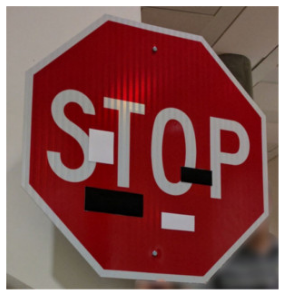
\includegraphics[width = \textwidth]{AdversarialStopSign-1707-08945}
% \column{.6\textwidth}
% \centering
% 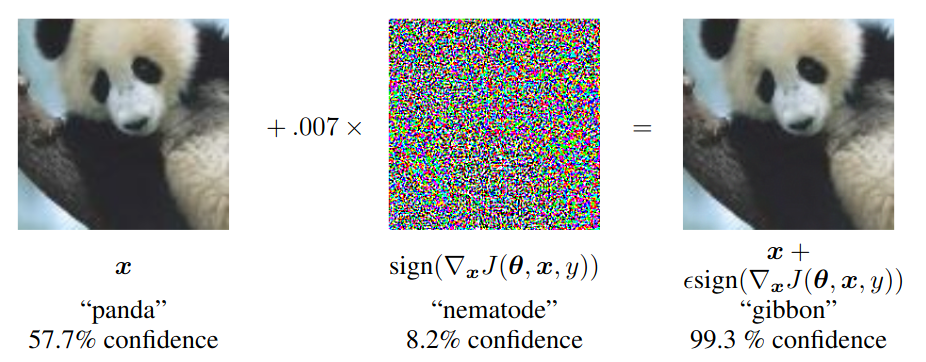
\includegraphics[width = \textwidth]{AdversarialAI-Panda}
% \vspace{1in}
% \end{columns}

% \bvfill
% Images from: \url{arxiv.org/abs/1707.08945}, \url{arxiv.org/abs/1412.6572}
% \end{frame}


{
  \setbeamercolor{background canvas}{bg=Apricot!25}
\begin{frame}
\bvfill
Determine whether each scenario is prediction, inference, or both.
\bvfill

\centering
\begin{tabular}{c|cc}
	\textbf{Application} & \textbf{Prediction} & \textbf{Inference}\\\hline
	Predict effectiveness of vaccine\\
	\\
	Determine the address written on\\
	the image of an envelope. \\
	\\
	Identify risk factors for getting long covid.\\
	\\
	Transcribe an audio file of a person talking. \\
	\\
	Predict stock prices. 
\end{tabular}

\bvfill


\end{frame}
}
%--- Next Frame ---%

% \section{Is there an ideal $f(X)$?}



\section{How to estimate $f$?}

\begin{frame}[c]{Input: Training data}

\begin{columns}
\column{.5\textwidth}
\begin{itemize}
	\item $n$ data points observed
	\item $x_{ij}$ is the $j$th predictor for observation $i$
	\item $y_i$ is the response variable for the $i$th observation
	\item Training data:
	\begin{itemize}
		\item $\{(x_1,y_1), (x_2,y_2), \cdots, (x_n,y_n)$
		\item $x_i = (x_{i},x_{i2},\cdots,x_{ip})^T$
	\end{itemize}
\end{itemize}
\column{.3\textwidth}
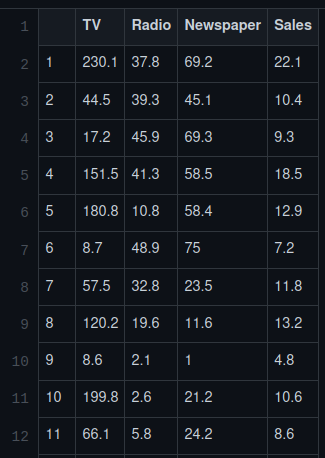
\includegraphics[alt={screenshot of the advertising data set},width = \textwidth]{AdvertisingDataSet-Screenshot}
\end{columns}

\end{frame}
%--- Next Frame ---%
\begin{frame}[c]{Parametric methods}

\begin{columns}
\column{.4\textwidth}
\begin{itemize}
	\item [\textbf{Step 1:}] Select a model

\qquad

	Example:
	\begin{equation*}
		f(X) = \beta_0 + \beta_1X_1 + \beta_2 X_2 + \cdots + \beta_pX_p
	\end{equation*}

	\item [\textbf{Step 2:}] Train the model

	\qquad

	Example:

	Find $\beta_i's$ so that
	\begin{equation*}
		Y \approx \beta_0 + \beta_1X_1 + \beta_2 X_2 + \cdots + \beta_pX_p
	\end{equation*}

\end{itemize}
\column{.4\textwidth}

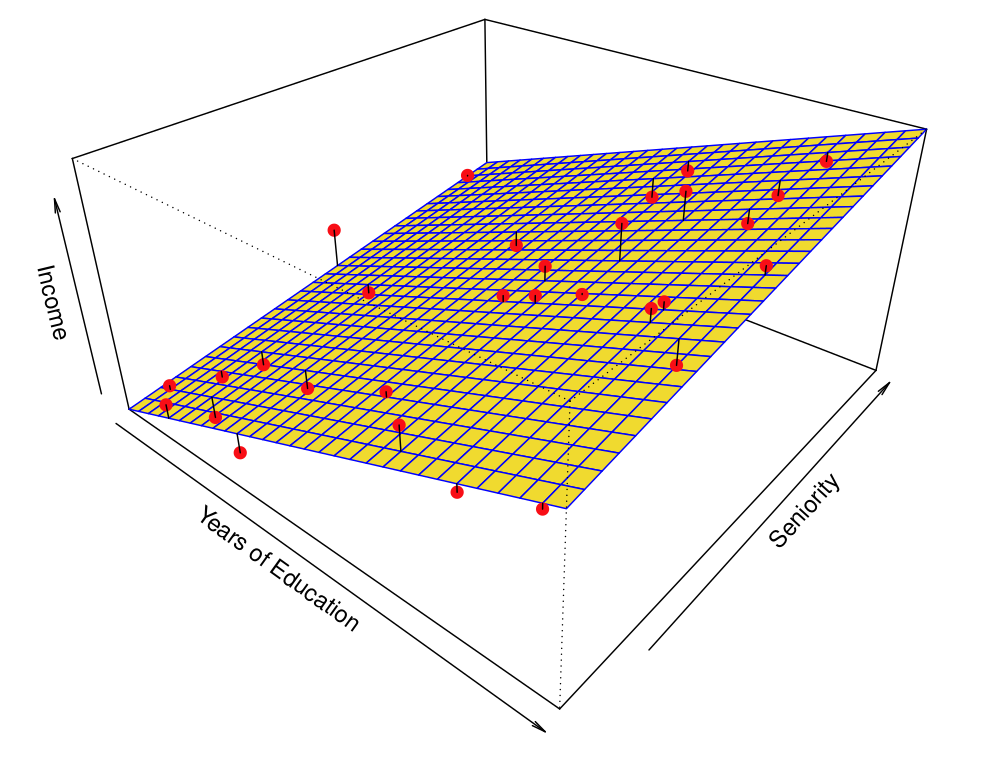
\includegraphics[alt={Data points for income in units of 1000 versus years of education and seniority along with a planar surface fit to data},width=\textwidth]{Fig2-4}
\end{columns}

\end{frame}
%--- Next Frame ---%
\begin{frame}[t]{How do you decide on the coefficients?}
\begin{columns}
\column{.45\textwidth}
\centering
\begin{equation*}
	Y \approx \beta_0 + \beta_1X_1 
\end{equation*}
\column{.45\textwidth}
\centering
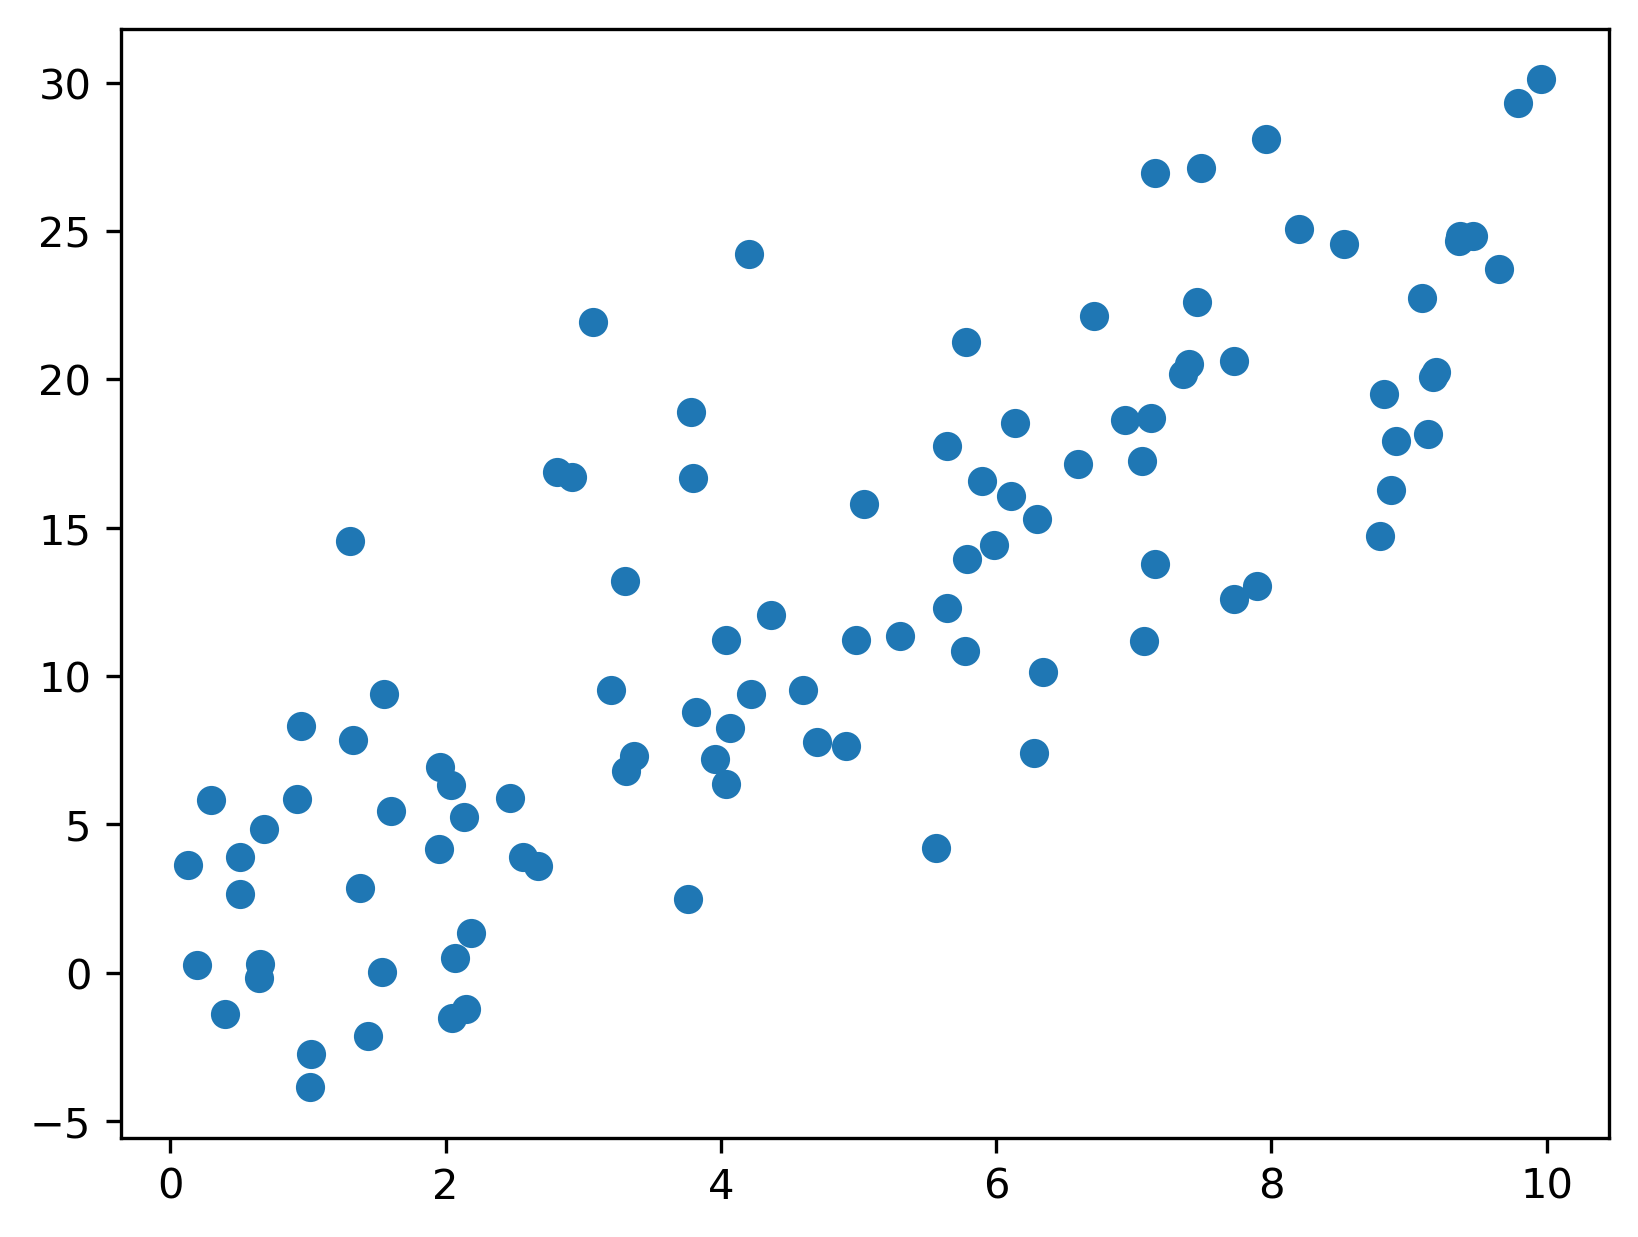
\includegraphics[alt={A 2D scatter plot},align = c, width = \textwidth]{ExampleScatter}

\end{columns}
\bvfill
Desmos toy: \url{https://www.desmos.com/calculator/skvt8c73l7}
\end{frame}
%--- Next Frame ---%

\begin{frame}[c]{Example Non-parametric method: Nearest Neighbors}

\begin{columns}
\column{.4\textwidth}
\centering
\begin{equation*}
	N_k(x) = \text{Set of $k$ nearest neighbors of $x$}
\end{equation*}
\begin{equation*}
	\hat f(x) = \frac{1}{k} \sum_{x_i \in N_k(x) } y_i
\end{equation*}
\vspace{1in}
\column{.4\textwidth}
\centering
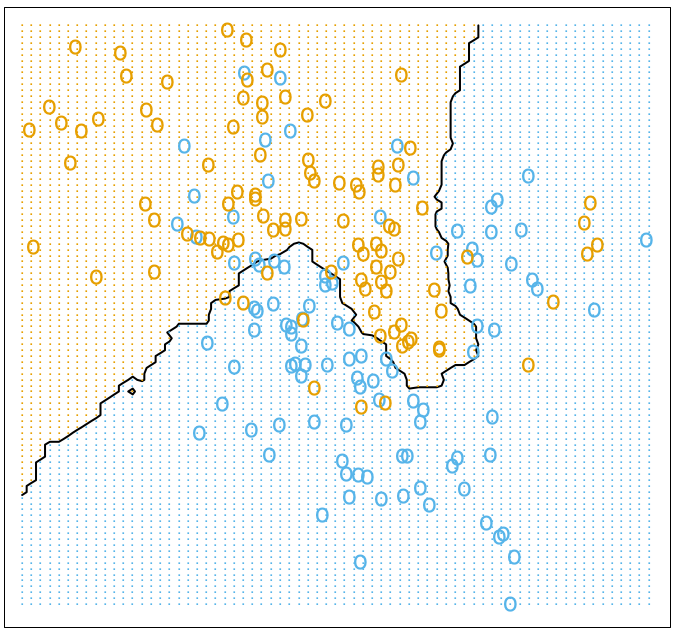
\includegraphics[alt={A picture of data with two classes separated by a non-linear boundary obtained using nearest neighobrs},width = \textwidth]{ESLR-Fig2-2.png}

$k = 15$
\end{columns}

\end{frame}
%--- Next Frame ---%
\begin{frame}[c]{Parametric methods: Pros and Cons}

\begin{columns}
\column{.4\textwidth}
\centering
\textbf{Pros}
\InstructorList{
\item Easier to estimate parameters than to figure out a completely arbitrary function
}
\column{.4\textwidth}
\textbf{Cons}
\centering
\InstructorList{
\item You might have chosen the wrong function type
}
\end{columns}
\bvfill


\end{frame}
%--- Next Frame ---%

\begin{frame}[c]{Overfitting}
\InstructorNotes{Possible fix: Find more \textbf{Flexible} models, which means braider functional form}

\InstructorNotes{Problem: needs more variables, could lead to overfitting}

\InstructorNotes{Overfitting: Following the noise too closely }

\begin{columns}
\column{.4\textwidth}
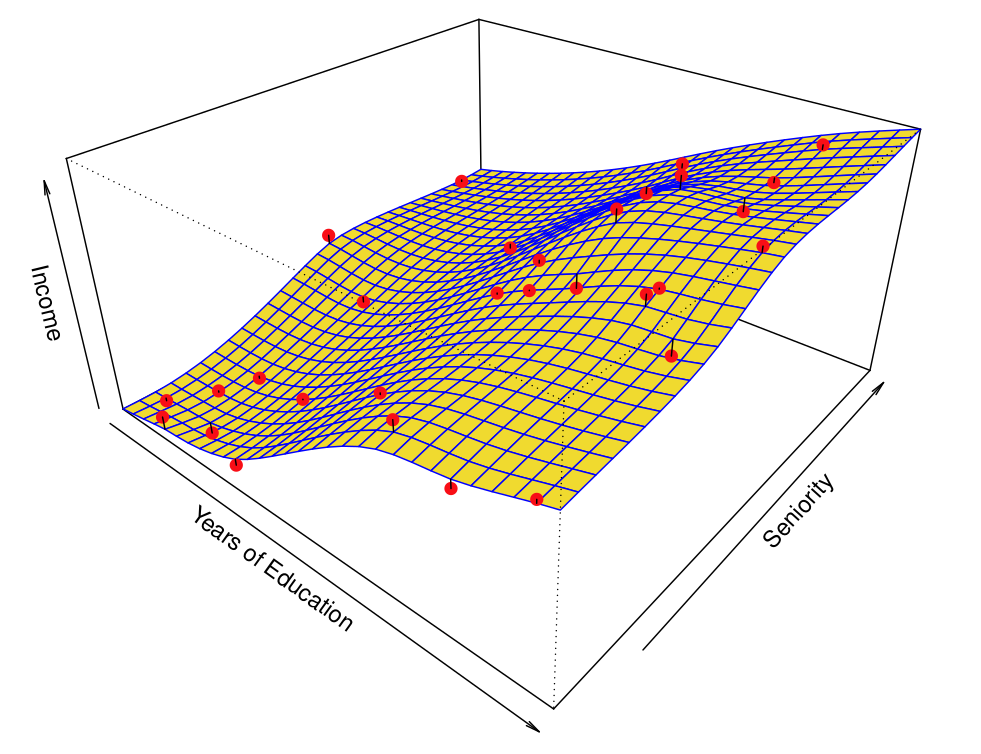
\includegraphics[alt={Data points for income in units of 1000 versus years of education and seniority along with a non-planar surface fit to data},width=\textwidth]{Fig2-5}
\column{.4\textwidth}
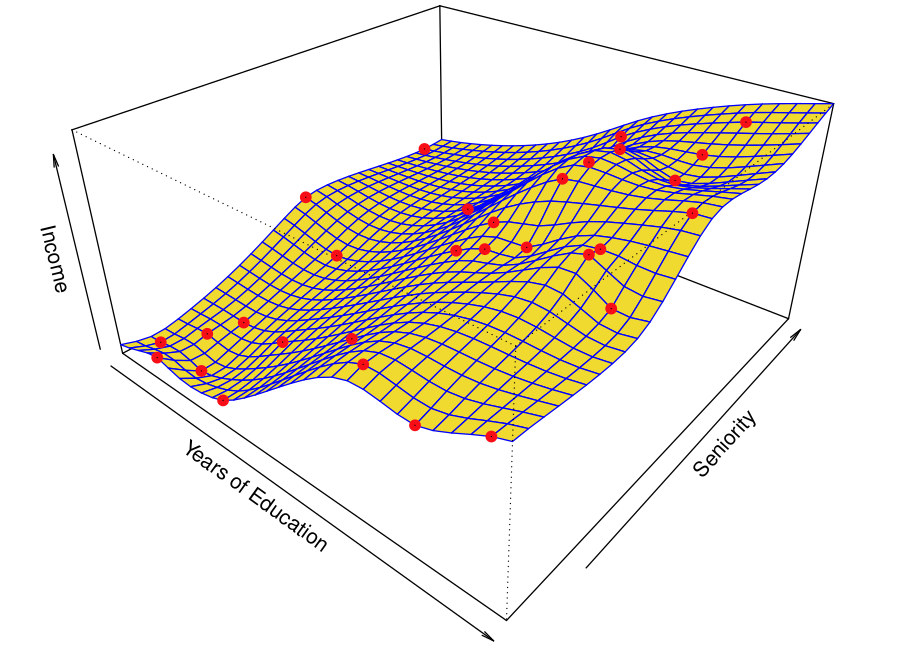
\includegraphics[alt={Data points for income in units of 1000 versus years of education and seniority along with a more flexible non-planar surface fit to data},width=\textwidth]{Fig2-6}

\end{columns}

\end{frame}
%--- Next Frame ---%

% \section{}


\begin{frame}[c]{Prediction Accuracy vs Model Interpretability }

\begin{columns}
\column{.7\textwidth}

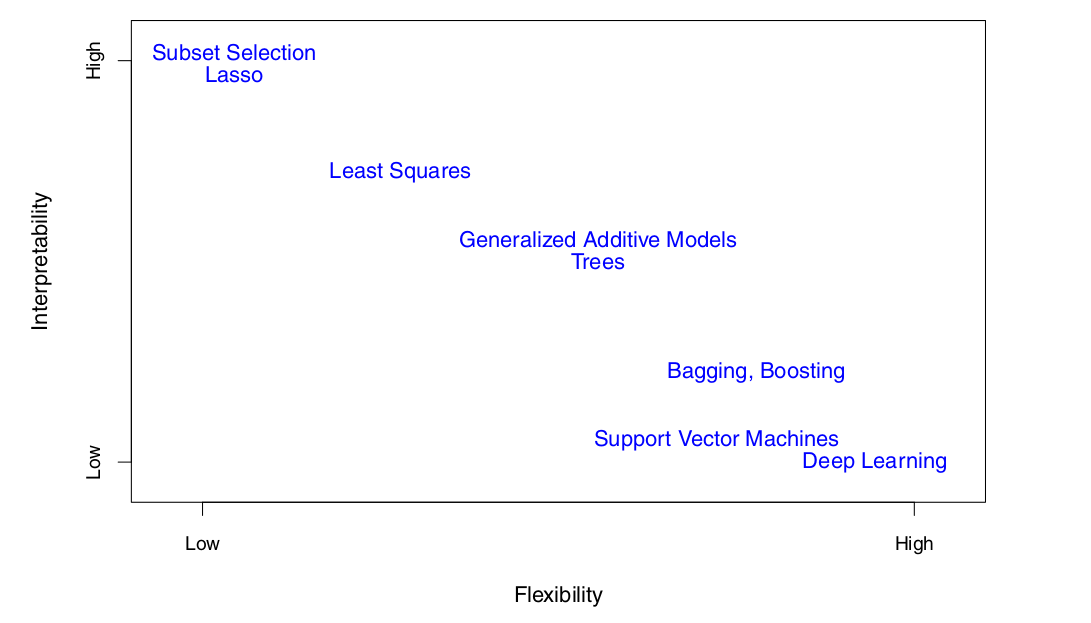
\includegraphics[alt={A figure that plots common methods for machine learning with low and high levels for interpretability on the y-axis versus flexiblity on the x-axis},
width=\textwidth]{Fig2-7}
\column{.3\textwidth}
\InstructorList{
\item More flexible allows for greater accuracy, but potential for overfitting
\item Also more restrictive makes it easier to understand and interpret the results
}

\end{columns}

\end{frame}
%--- Next Frame ---%




\begin{frame}


\begin{columns}
\column{.4\textwidth}
\textbf{Supervised learning:}\\
Training data has response variable $y$ for every input $x$

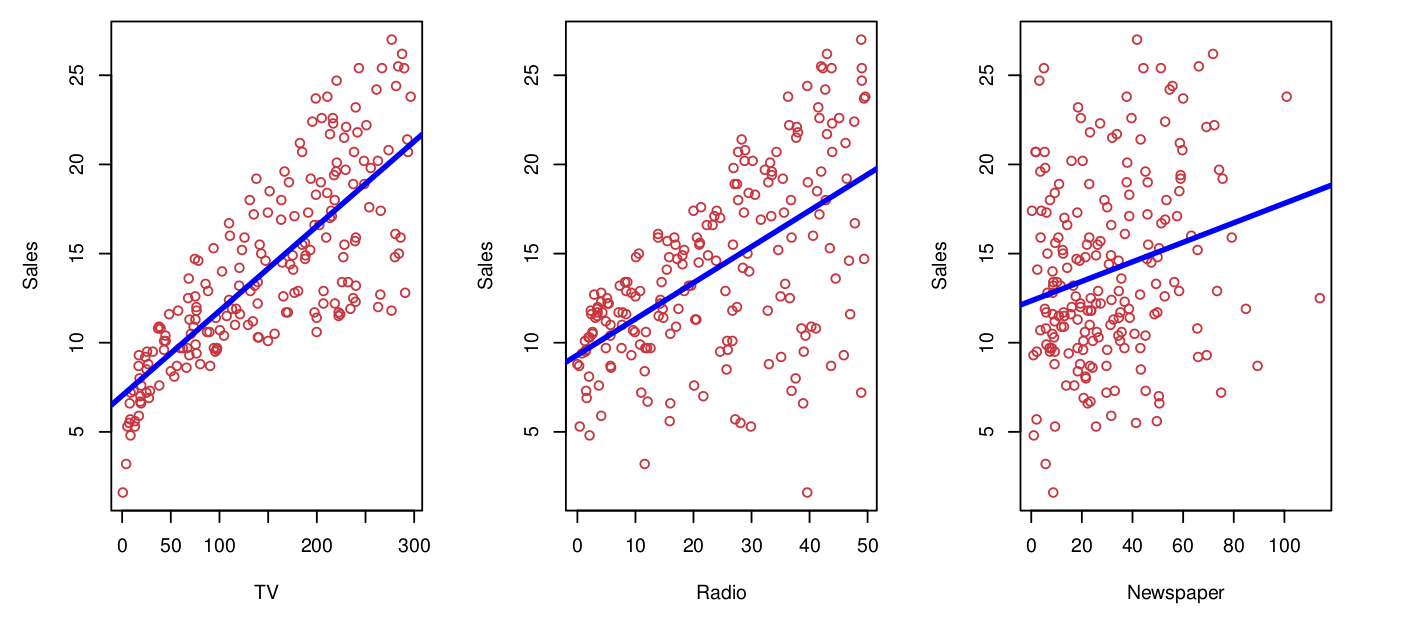
\includegraphics[alt={Sales versus TV, radio, and newspaper advertising spending all in units of 1000},height = 2.3in,trim = 0 0 950 0, clip]{Fig2-1}


\column{.4\textwidth}
\textbf{Unsupervised Learning:}\\
Training data does not have response variable $y$ for every input $x$

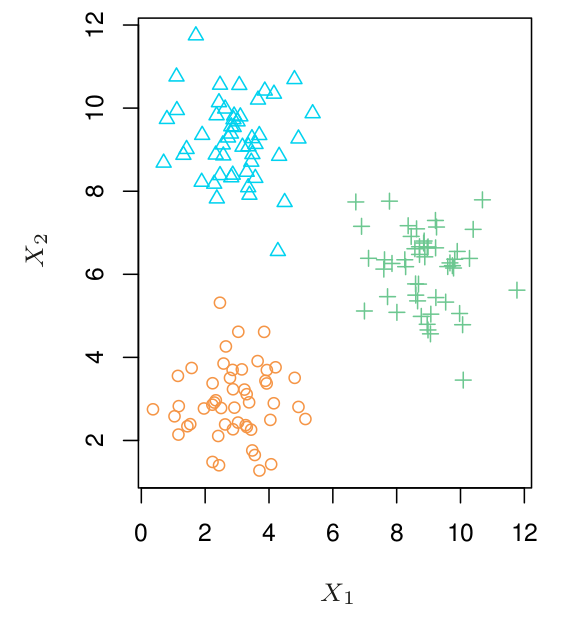
\includegraphics[alt={Plot of 3 different classes separately grouped versus two predictors X1 and X2},height = 2.3in]{Fig2-8a}
\end{columns}

\end{frame}
%--- Next Frame ---%


\begin{frame}[c]{Regression vs Classification}


\begin{columns}
\column{.4\textwidth}
\textbf{Types of variables:} \InstructorNotes{Emphasize this is output variable, and which it is determines regression vs classification}

\begin{itemize}
	\item Quantitative

\InstructorNotes{Ex: Blood pressure, temperature, volume, height, income}
	\vspace{1in}

	\item Qualitative / Categorical

\InstructorNotes{Purchased a ticket, owns a house, Job, Digit in MNIST, }

	\vspace{ 1in}
\end{itemize}
\column{.4\textwidth}

\end{columns}

\InstructorNotes{Emphasize that this has to do with the output variable type}

\end{frame}
%--- Next Frame ---%

\section{Group work}
{
  \setbeamercolor{background canvas}{bg=Apricot!40}
\begin{frame}
\begin{columns}
\column{.4\textwidth}
(a) We collect a set of data on the top 500 firms in the US. For each
firm we record profit, number of employees, industry and the
CEO salary. We are interested in understanding which factors
affect CEO salary.
\column{.5\textwidth}

\begin{itemize}
	\item Is this classification or regression? 
	\InstructorNotes{regression}
	\item Do we want inference or prediction?
	\InstructorNotes{Inference}
	\item What is $n$, the number of data points?
	\InstructorNotes{500}
	\item What is $p$, the number of variables?
	\InstructorNotes{3}
\end{itemize}
\end{columns}

% \bvfill
	\InstructorNotes{From Ex 2.4.2}
\end{frame}
%--- Next Frame ---%

\begin{frame}
\begin{columns}
\column{.4\textwidth}
(b) We are considering launching a new product and wish to know
whether it will be a success or a failure. We collect data on 20
similar products that were previously launched. For each product we have recorded whether it was a success or failure, price
charged for the product, marketing budget, competition price,
and ten other variables.
\column{.5\textwidth}
\begin{itemize}
	\item Is this classification or regression?
	\InstructorNotes{classification}
	\item Do we want inference or prediction?
	\InstructorNotes{Prediction}
	\item What is $n$, the number of data points?
	\InstructorNotes{20}
	\item What is $p$, the number of variables?
	\InstructorNotes{13}
\end{itemize}
\end{columns}

\end{frame}
}
%--- Next Frame ---%
\begin{frame}[t]{TL;DR}
\begin{columns}
\column{.45\textwidth}
\centering


\InstructorList{
	\item Input/output variables
	\item Prediction vs inference
	\item Reduceable vs irreduceable error
	\item Overfitting
	\item Classification vs regression
	\item Supervised vs Unsupervised learning
}

\column{.45\textwidth}
\centering
\end{columns}
\end{frame}
%--- Next Frame ---%
\begin{frame}[c]{Wrap up }

\begin{columns}
\column{.4\textwidth}
\centering

\textbf{Next time:}
	\begin{itemize}
		%\item Friday 8/30 and Monday 9/2
		%\begin{itemize}
			%\item NO CLASS!!!!
		%\end{itemize}
		\item Friday 1/16
		\begin{itemize}
			% \item Assessing Model Accuracy
			\item Bring Laptop!
			\item First homework due Sun Jan 25
			\item There will be a quiz this Friday
		\end{itemize}


	\end{itemize}
	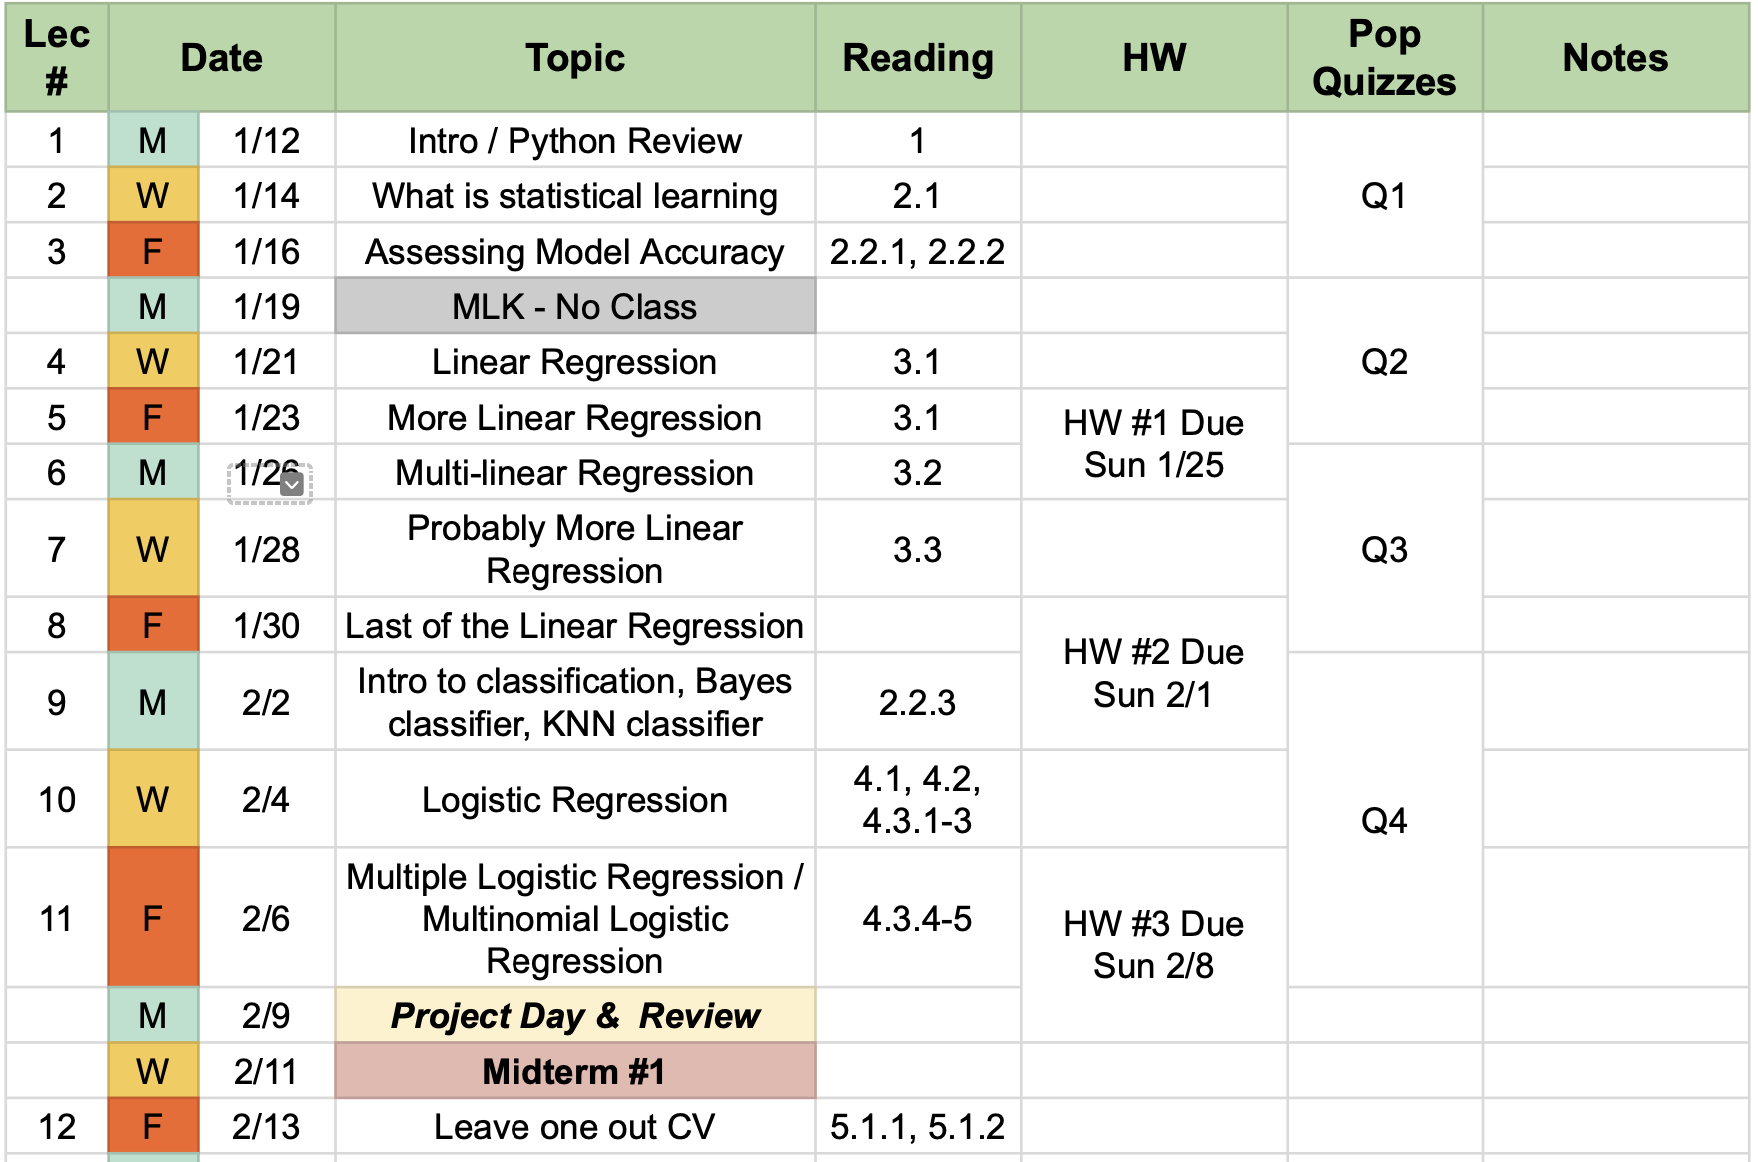
\includegraphics[alt={screenshot of course class schedule for lectures 1 to 12},align = c, width = .7\textwidth, trim = 0 170 0 0, clip]{Schedule-S26-1.png}
\column{.5\textwidth}
\centering

	\textbf{Announcements:}
	\begin{itemize}
		%\item Get on slack!
		%\begin{itemize}
		%	\item +1 point on the first homework if you post a gif in the thread
		%\end{itemize}
		\item Office hours!
		\begin{itemize}
			\item Dr.~Bao: Tue 9 am-11 am (EB 2507 L)\\
			\item Dr.~ Khasawneh: MWF 13:40 pm-2:00 pm (EB 2400), Tue 1:30 pm-2:30 pm (Zoom)
			% (At least this week, subject to change)
			\item Siyu : Wed 2:00 pm-3:00 pm (EB 2504)
			\item Haishen: WF 2:00 pm-3:00 pm (EB2504)
		\end{itemize}
	\end{itemize}
\end{columns}

\end{frame}
%--- Next Frame ---%


\end{document}
